\begin{frame}[fragile]{Empirical Evaluation}
  \begin{block}{Research Questions}
    \begin{itemize}
          \item Does $\dpwcc$ in Haskell support the dynamic parallelization level that $\dpwcc$ requires?
          \item Is $\dpwcc$ in Haskell competitive compared with default implementations on base libraries for the same problem?
          \item Does $\dpwcc$ in Haskell handle memory efficiently?
      \end{itemize}        
  \end{block}
  \begin{block}{Experiments}
    \begin{itemize}
      \item \textbf{Implementation Analysis}: Measure and analyze Total execution time, MUT time and GC Time.
      \item \textbf{Benchmark Analysis}: Compare $DP_{WCC}$ with \mintinline{haskell}{Data.Graph} $WCC$ execution times:
      \begin{itemize}
        \item Using \mintinline{haskell}{ criterion } library.
        \item Diefficency metric $\mathtt{dief@t}$ (\textit{diepfy} tool) to measure incremental results.
      \end{itemize}
      \item \textbf{Performance Analysis}: Thread and Memory allocation analysis.
    \end{itemize}
  \end{block}
\end{frame}

\begin{frame}[fragile]{Empirical Evaluation}
  \begin{block}{Graphs Tested}
  \begin{table}[H]
    \centering
    \begin{tabular}{|p{0.25\linewidth}|r|r|r|p{0.25\linewidth}|}
     \hline
     \textbf{Network} & \textbf{Nodes} & \textbf{Edges} & \textbf{\#WCC} & \textbf{\#Nodes Largest WCC} \\
     \hline
     Enron Emails & 36692 & 183831 & 1065 & 33696 (0.918) \\
     \hline
     Astro Physics Collaboration Net & 18772 & 198110 & 290 & 17903 (0.954)\\
     \hline
     Google Web Graph & 875713 & 5105039 & 2746 & 855802 (0.977)\\
     \hline
    \end{tabular}
   \end{table}
  \end{block}
  \begin{block}{Hardware Environment}
    \begin{itemize}
          \item $x86$ $64$ bits
          \item $6$-Core Intel Core i7 processor of $2,2$ GHz up to $12$ virtual cores
          \item \emph{Hyper-threading} enable
          \item $32 GB$ \emph{DDR4} of RAM, $256\ KB$ of L2 cache memory, and $9\ MB$ of L3 cache
      \end{itemize}        
  \end{block}
\end{frame}

\begin{frame}[fragile]{Empirical Evaluation}
  \frametitle{Diefficiency Metrics}
    \begin{figure}[!htb]
      \centering
      \begin{minipage}{0.33\textwidth}
       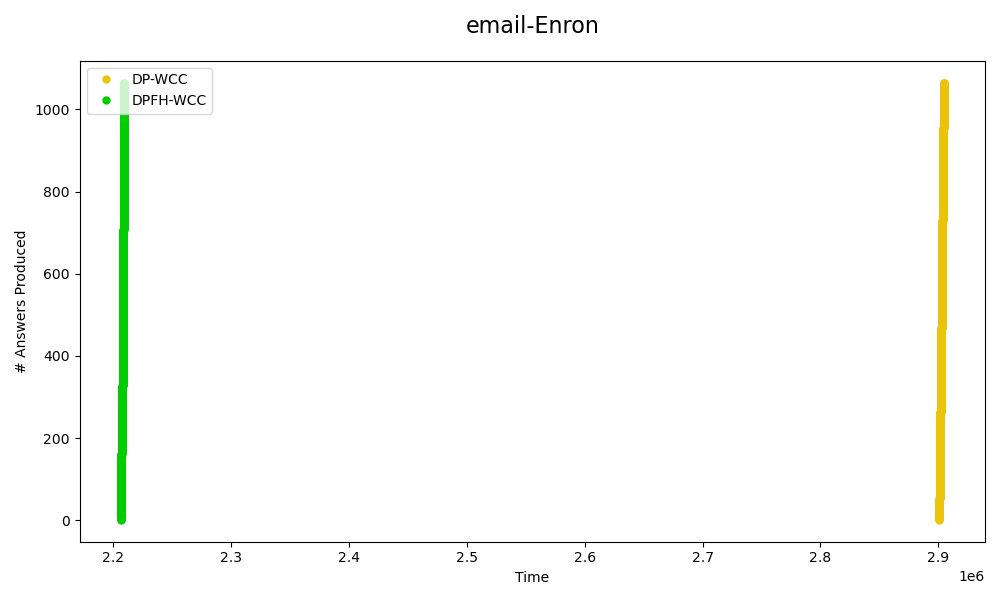
\includegraphics[width=1\linewidth, height=0.4\textheight]{email_enron}
      \end{minipage}%
      \begin{minipage}{0.33\textwidth}
       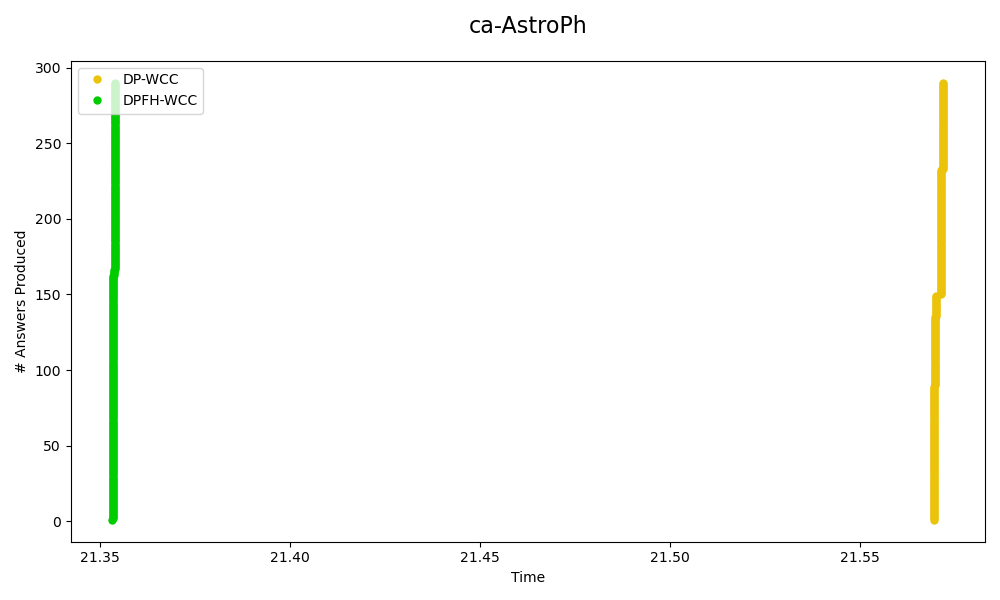
\includegraphics[width=1\linewidth, height=0.4\textheight]{ca_astroph}
      \end{minipage}%
      \begin{minipage}{0.33\textwidth}
       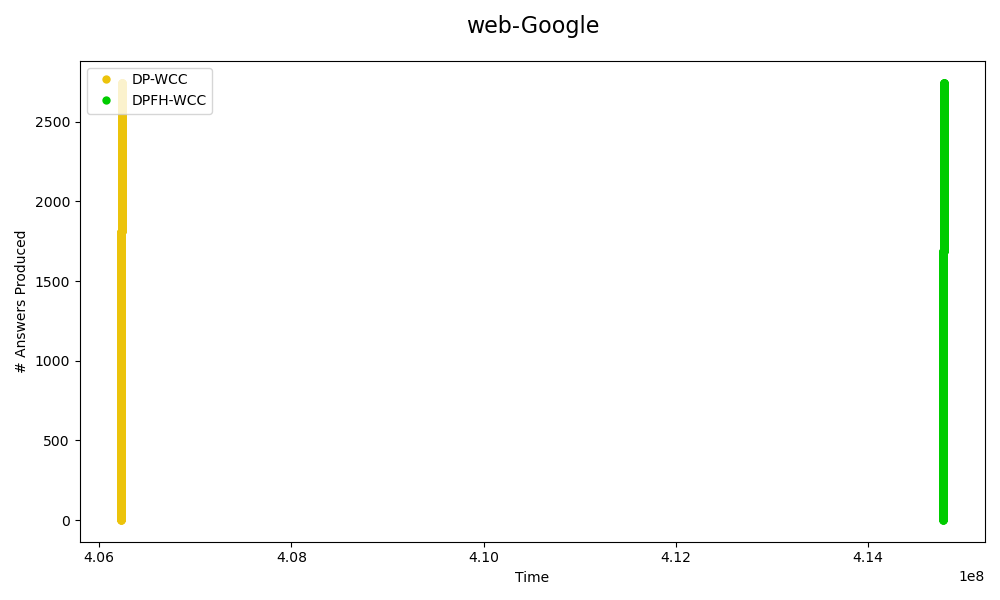
\includegraphics[width=1\linewidth, height=0.4\textheight]{web_google}
      \end{minipage}
  \end{figure}
\begin{figure}[!htb]
    \centering
    \begin{minipage}{0.33\textwidth}
     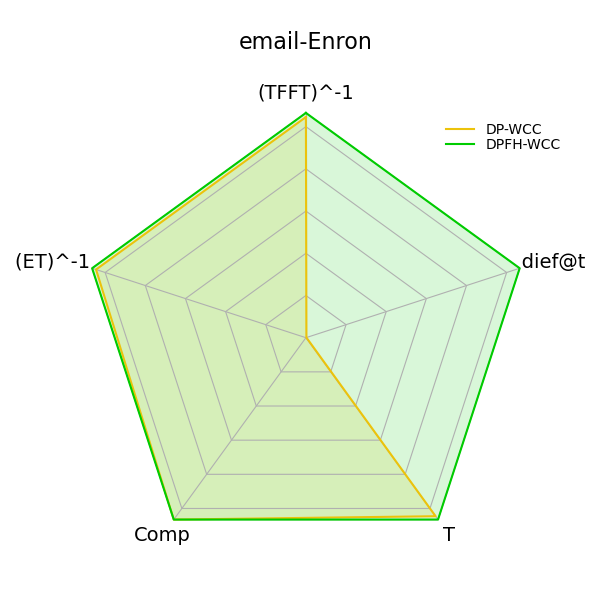
\includegraphics[width=1\linewidth, height=0.35\textheight]{email_enron_radar}
    \end{minipage}%
    \begin{minipage}{0.33\textwidth}
     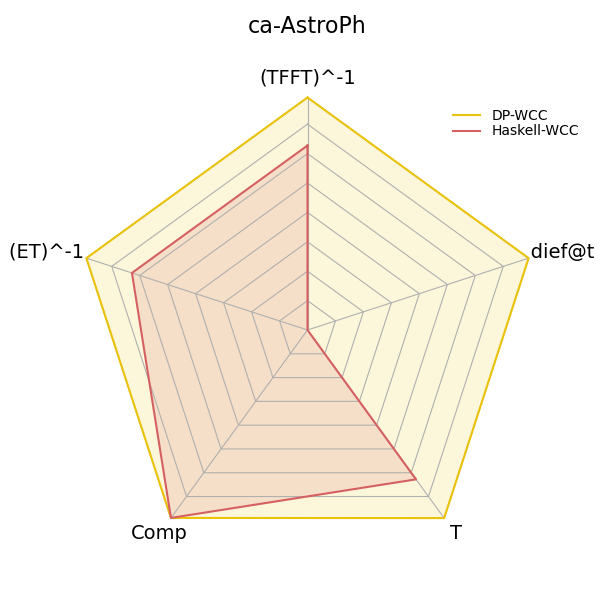
\includegraphics[width=1\linewidth, height=0.35\textheight]{ca_astroph_radar}
    \end{minipage}%
    \begin{minipage}{0.33\textwidth}
     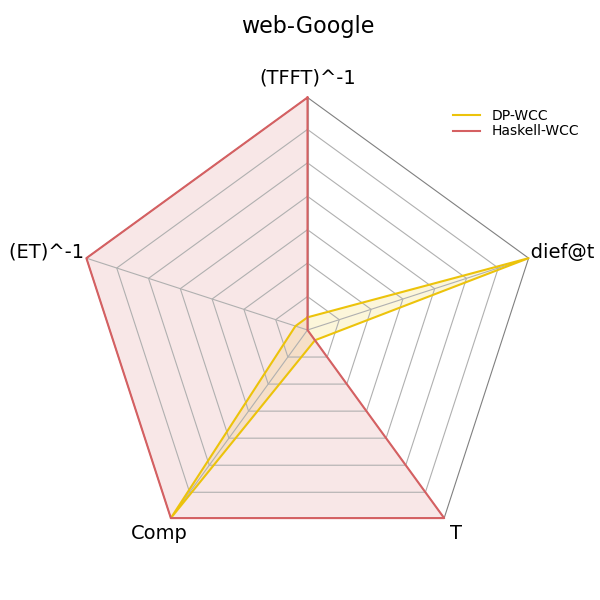
\includegraphics[width=1\linewidth, height=0.35\textheight]{web_google_radar}
    \end{minipage}
\end{figure}
\end{frame}

\begin{frame}[fragile]{Empirical Evaluation}
  \frametitle{Benchmark}

  \begin{block}{Execution time}
  \begin{table}[H]
    \centering
    \begin{tabular}{|l|l|l|l|}
     \hline
     \textbf{Network} & \textbf{DP-Haskell} & \textbf{Data.Graph} & \textbf{Speed-up}\\
     \hline
     Enron Emails & 4.68s &  6.46s & 1.38\\
     \hline
     Astro Physics Coll Net & 4.98s & 6.95s  & 1.39\\
     \hline
     Google Web Graph & 386s & 106s & \color{red}0.27\\
     \hline
    \end{tabular}
   \end{table}      
  \end{block}

   \vspace{1cm}

  \begin{minipage}[t]{\linewidth}
    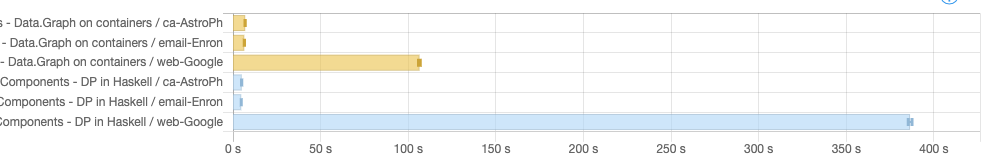
\includegraphics[width=\textwidth]{bench_2}
  \end{minipage}
\end{frame}

\begin{frame}[fragile]{Empirical Evaluation}
  \begin{columns}[onlytextwidth] 
    \begin{column}{.45\textwidth} 
      \begin{block}{ThreadScope}
        \begin{minipage}{\textwidth}
          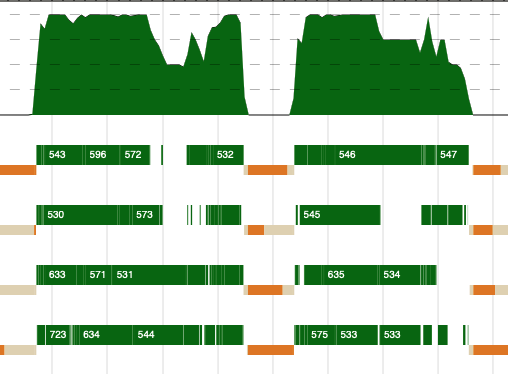
\includegraphics[width=1\linewidth, height=0.5\textheight]{screen_2}
        \end{minipage}%     
      \end{block}%
    \end{column} \hfill%
    \begin{column}{.45\textwidth} 
      \begin{block}{Eventlog - Memory Allocation}
        \begin{minipage}{\textwidth}
          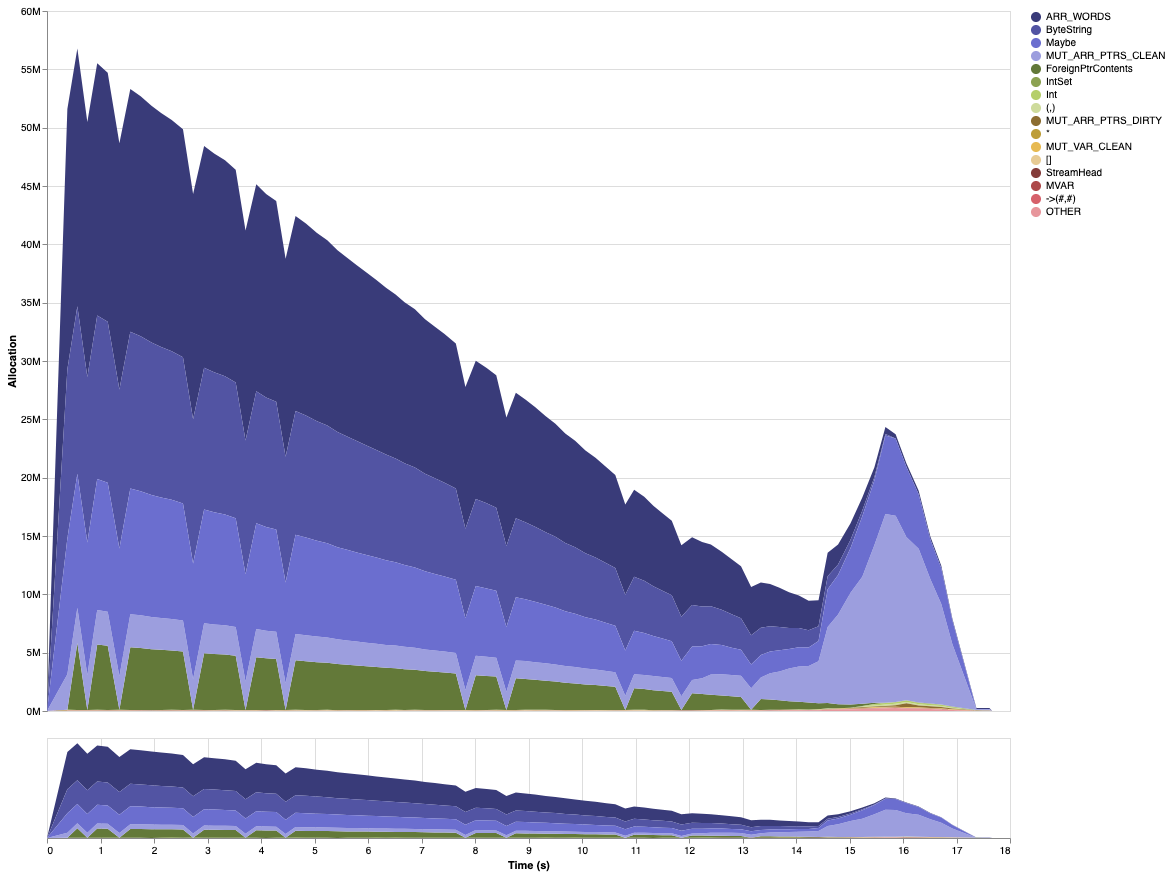
\includegraphics[width=1\linewidth, height=0.5\textheight]{visualization}
        \end{minipage}%
      \end{block}
  \end{column} 
\end{columns}
\end{frame}
